\chapter{Evaluatie van integratie methoden}
\label{cha:D:evaluatie}

\section{Introductie}
\label{sec:D:evaluatie-introductie}
In dit hoofdstuk zullen we onderzoeken of de verschillende integratie strategie\"en en impact hebben op de performantie van de resulterende modellen. We doen dit door in twee concrete case studies, op echte kankergegevens, een model uit te werken gebruikmakend van elke strategie. En vervolgens de bekomen modellen te evalueren met een passende metriek.

\section{Case studie 1: logistieke regressie}
\subsection{Case overzicht}
In de eerste case studie zullen we logistieke regressie modellen gebruiken. De gebruikte datasets komen van het Universitair Ziekenhuis te Leuven en betreffen gegevens van pati\"enten met darmkanker. Van deze pati\"enten zijn tijdens de behandeling scans genomen met een MRI scanner, PET scanner en DWI scanner. We hebben in dit geval dus te maken met drie datasets. De output variabele die we zullen trachten te voorspellen is een binaire versie van het pathologisch stadium van elke pati\"ent (zie appendix \ref{app:cancer-staging}). We kunnen stellen dat pati\"enten met een label 1 van de kanker zijn genezen, en pati\"enten met een label 0 niet. Deze output die het predictief model ons zal geven is dus een kans op genezing.
\subsection{Evaluatie methode}
We zullen de logistieke modellen evalueren met een Receiver-Operator Characteristic analyse. Herinner je dat we via cross-validatie voor elk datapunt in onze dataset een predictie konden bekomen. In het geval van logistieke regressie is deze predictie een probabiliteit. De output voor de datapunten in onze dataset zijn echter binaire waarden (de realisaties van de binomiaalverdeling). Om de twee te kunnen vergelijken moeten we een drempelwaarde defini\"eren. Als de voorspelde probabiliteit hoger is dan deze drempelwaarde dan voorspellen we een positieve output, anders een negatieve output. Voor elk datapunt zijn er hierbij dan vier scenario's mogelijk:
\begin{itemize}
	\item True Positive (TP): het model voorspelt een positieve output, en dat is correct
	\item True Negative (TN): het model voorspelt een negatieve output, en dat is correct
	\item False Positive(FP): het model voorspelt een positieve output, en dat is fout (type 1 fout)
	\item False Negative (FN): het model voorspelt een negatieve output, en dat is fout (type 2 fout)
\end{itemize}
Merk op dat we in dit geval niet enkel zeggen of het model juist of fout was, maar ook de type fout registreren. Dit laat ons toe om volgende begrippen van sensitiviteit en specificiteit te defini\"eren:
$$
sensitiviteit = \frac{\sum{TP}}{\sum{P}}
$$
$$
specificiteit = \frac{\sum{TN}}{\sum{N}}
$$
hierin zijn
\begin{itemize}
	\item $\sum{TP}$ het totale aantal true positives
	\item $\sum{P}$ is het totale aantal datapunten met positieve output in de dataset
	\item $\sum{TN}$ het totale aantal true negatives
	\item $\sum{N}$ is het totale aantal datapunten met negatieve output in de dataset
\end{itemize}
Het perfecte model, dat altijd juist voorspelt, heeft een sensitiviteit en specificiteit gelijk aan 1. In een realistische setting is dit echter zelden haalbaar. We willen beide metrieken echter zo dicht mogelijk bij 1. We kunnen nu een plot maken waarbij we op de sensitiviteit plotten in functie van de specificiteit voor verschillende waarden van de drempelwaarde. Merk op dat inderdaad verschillende drempelwaarden ervoor zullen zorgen dat het model verschillende voorspellingen maakt en dus sensitiviteit en specificiteit zullen be\"invloeden. De curve die we bekomen op deze plot noemt men een Receiver Operating Characteristic curve. Een voorbeeld curve wordt getoont op figuur \ref{fig:D:evaluation-roc}. De metriek die we zullen gebruiken is de oppervlakte onder deze ROC curve, ook wel afgekort AUC(Area Under the ROC Curve). Hoe hoger deze waarde, hoe groter de waarden voor sensitiviteit en specificiteit bij verschillende drempelwaarden, en dus hoe beter ons predictief model.
\begin{figure}
	\centering
	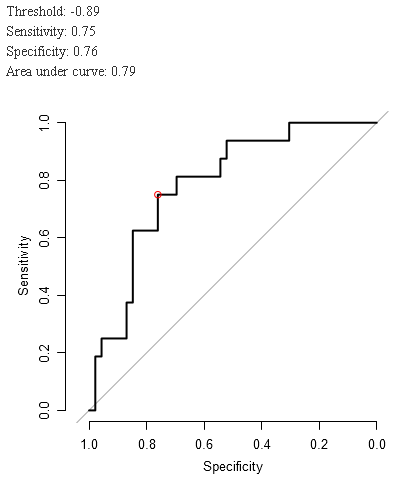
\includegraphics[scale=.7]{images/roc_curve}
	\caption{Voorbeeld ROC curve en metrieken}
	\label{fig:D:evaluation-roc}
\end{figure}

\section{Resultaten}
De resulterende AUC waarden worden getoond in tabellen \ref{tab:D:evaluation-auc-individual} en \ref{tab:D:evaluation-auc-integrated}, respectievelijk voor modellen op individuele datasets, en ge\"integreerde modellen.
Uit de eerste tabel is het duidelijk dat de MRI dataset de meeste predictieve informatie bevat. Maar door gebruik te maken van integratie technieken kunnen we duidelijk de performantie van de modellen verbeteren. Tevens kunnen we opmerken dat, onafhankelijk van de gebruikte datasets, de parti\"ele integratie de beste methode blijkt in dit geval.
\begin{table}
	\centering
	\begin{tabular}{lc}
		\toprule
		Dataset & AUC \\
		\midrule
		DWI & 0.67 \\
		MRI & 0.75 \\
		SUV & 0.65 \\
		\bottomrule
	\end{tabular}
	\caption{AUC voor modellen getraind op individuele datasets}
	\label{tab:D:evaluation-auc-individual}
\end{table}
\begin{table}
	\centering
	\begin{tabular}{lcccc}
		\toprule
		& Alle datasets & DWI+MRI & DWI+SUV & MRI+SUV \\
		\midrule
		Vroege integratie & 0.76 & 0.82 & 0.69 & 0.74 \\
		Parti\"ele integratie & 0.79 & 0.83 & 0.78 & 0.75 \\
		Late integratie & 0.73 & 0.78 & 0.66 & 0.70 \\
		\bottomrule
	\end{tabular}
	\caption{AUC voor ge\"integreerde modellen voor verschillende combinaties van de datasets}
	\label{tab:D:evaluation-auc-integrated}
\end{table}
\section{Case studie 2: cox proportionele risico modellen}
\subsection{Case overzicht}
In de tweede case studie zullen we cox modellen gebruiken. De gebruikte datasets komen in dit geval van The Cancer Genome Atlas. Dit is een project van het National Cancer Institute waarbij 2.5 petabytes aan gegevens werden publiek gemaakt over pati\"enten met 33 types van kanker. Hiervan zullen we gebruik maken van enkele datasets voor keelkanker pati\"enten. Meerbepaald de datasets met Copy Number Variaties, messenger RNA data en micro RNA data. Dit zijn drie datasets die aanwijzingen geven over defecten in het DNA. We zullen deze gegevens proberen te correleren met de overlevingskans van pati\"enten gebruikmakend van het cox model.
\subsection{Evaluatie methode}
Om de overlevingsmodellen te evalueren zullen we gebruik maken van een significantie test genaamd de Wald Test. Een significantie test vergelijkt het bekomen model met een ander hypothetisch model genaamd de null-hypothese. In dit geval is de null-hypothese het overlevingsmodel waarbij alle gewichten (de parameters van ons model) gelijk zijn aan 0. Dit zou willen zeggen dat geen enkele van de variabelen in de datasets een impact heeft op de overleving (of op het risico tot overlijden) van de pati\"enten. Een significantie-test is bedoeld om aan te tonen dat deze null-hypothese te verwerpen is, namelijk dat de gegevens die geobserveerd worden heel erg onwaarschijnlijk zijn, in het geval dat de null-hypothese waar is. Als we die onwaarschijnlijkheid kunnen aantonen dan zeggen we dat we de null-hypothese verwerpen, en dat geeft aan dat het model dat we gevonden hebben significant is. De formule voor de Wald test waarbij 1 enkele variabele wordt getest is:
\begin{equation}
\begin{split}
\frac{(\hat{\beta}-\beta_{0})^{2}}{var(\hat{\beta})} \sim \tilde{\chi}^{2}_{1}
\end{split}
\end{equation}
where
\begin{itemize}
	\item $\hat{\beta}$ is de waarde voor de variabele die we zijn bekomen in ons model
	\item $\beta_{0}$ is de waarde van de variabele $\beta$ indien de null-hypothese waar is, in ons geval is dat de waarde 0.
	\item $var(\beta)$ is de variantie van de variabele $\beta$
	\item $\tilde{\chi}^{2}_{1}$ is de chi-kwadraat verdeling met 1 vrijheidsgraad
\end{itemize}
Wat de Wald test dus berekent is de afstand tussen de gevonden waarde, en de waarde onder de null-hypothese, relatief ten opzichte van de onzekerheid over de variabele (de variantie). Hoe groter de waarde van de Wald test, hoe significanter het model. Een schematische voorstelling wordt gegeven op figuur \ref{fig:D:evaluation-wald-test}. In de statistiek wordt deze waarde echter vaak omgevormd tot een p-waarde. De p-waarde is een waarde tussen 0 en 1 (het is een probabiliteit), en is berekenbaar uit de waarde van de Wald test. Het geeft dus geen enkele extra toegevoegde waarde, maar we tonen deze waarde omwille van zijn populariteit. Daarnaast is het ook veelvoorkomend om een drempelwaarde in te stellen voor de p-waarde. Indien de p-waarde lager ligt dan deze waarde beschouwen we het model als significant. Een veelgebruikte drempelwaarde is 0.05.
\begin{figure}
	\centering
	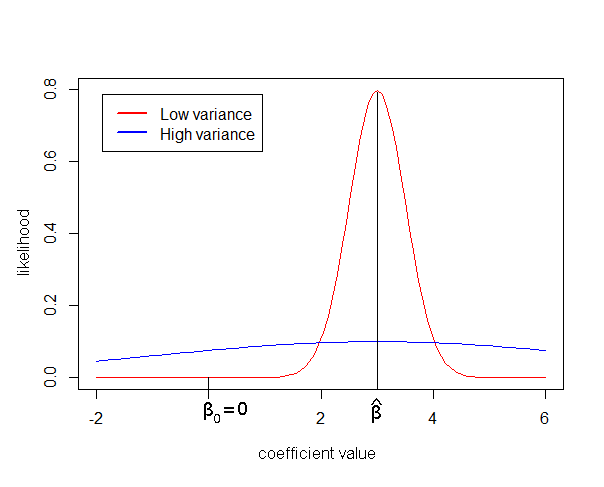
\includegraphics[scale=.7]{images/wald_test}
	\caption{Voorbeeld Wald test variantie visualisatie. Beide curves geven dezelfde maximum likelihood schatting voor $\hat{\beta}$. De rode curve heeft echter een lage variantie, wat veel evidentie biedt om de null-hypothese te verwerpen. De blauwe curve heeft een hoge variantie, in dit geval is het niet meteen duidelijk dat $\hat{\beta}$ echt verschilt van $\beta_{0}$ en dus kunnen we de null-hypothese niet verwerpen.}
	\label{fig:D:evaluation-wald-test}
\end{figure}

\section{Resultaten}
Tabel \ref{tab:D:evaluation-case2-dimensions} geeft een overzicht van de dimensies van de gebruikte datasets. De resultaten van de significantietests voor alle modellen worden getoond in de tabellen \ref{tab:D:evaluation-surv-individual} en \ref{tab:D:evaluation-surv-integrated}. Het is meteen duidelijk dat bijna alle modellen niet significant zijn. De berekende p-waarden zijn duidelijk ver boven de vooropgestelde grens van 0.05. Dat terzijde is het interessant om op te merken dat alle ge\"integreerde modellen duidelijk meer significant zijn dan de modellen voor individuele datasets. Meer nog, het partieel ge\"integreerde model is het enige model dat het significantie niveau van 0.05 bereikt. Er zou echter meer onderzoek moeten gebeuren om de werkelijke predictieve waarde van dit model te onderzoeken, maar voor deze studie is het duidelijk dat dit model het beste model is. En dus kunnen we concluderen dat de ge\"integreerde modellen ook hier aantonen dat ze een positieve impact hebben op de performantie van de bekomen modellen.
\begin{table}
	\centering
	\begin{tabular}{lcc}
		\toprule
		Dataset naam & Aantal variabelen & Aantal pati\"enten \\
		\midrule
		Copy Number Variations & 16 & 219\\
		messenger RNA & 3869 & 219 \\
		micro RNA & 414 & 219 \\
		\bottomrule
	\end{tabular}
	\caption{Dimensies voor de datasets die gebruikt werden in de overlevingsanalyse.}
	\label{tab:D:evaluation-case2-dimensions}
\end{table}

\begin{table}
	\centering
	\begin{tabular}{lccc}
		\toprule
		& CNV    & mRNA & miRNA \\
		\midrule
		Wald test 					& 0.17 & 0.13  & 1.46 \\
		P-waarde 					& 0.6799 & 0.7209  & 0.2276 \\
		\bottomrule
	\end{tabular}
	\caption{Significantie waarden voor de overlevingsmodellen voor individuele datasets}
	\label{tab:D:evaluation-surv-individual}
\end{table}

\begin{table}
	\centering
	\begin{tabular}{lccc} 
		\toprule
		& Early & Intermediate & Late\\
		\midrule
		Wald test 					& 2.43 & 3.89 & 1.98 \\
		P-waarde 					& 0.1192 & 0.0485 & 0.1595 \\
		\bottomrule
	\end{tabular}
	\caption{Significantie waarden voor de ge\"integreerde overlevingsmodellen}
	\label{tab:D:evaluation-surv-integrated}
\end{table}
%%% Local Variables: 
%%% mode: latex
%%% TeX-master: "thesis"
%%% End: 
